\documentclass{article}
\usepackage[utf8]{inputenc}
\usepackage[official]{eurosym}
\usepackage{graphicx}
\usepackage[font=small,labelfont=bf]{caption}

\newcommand{\size}{0.9\textwidth}

\newcommand{\image}[3]{
\begin{figure}
\begin{center}
\includegraphics[width=\size]{#1}
\caption{#2}
#3
\end{center}
\end{figure}
}

% New Packages
\usepackage{hyperref}
% Referenz
\newcommand{\secref}[1]{\autoref{#1}. \texit{\nameref{#1}}}

\usepackage{floatrow}
% Table float box with bottom caption, box width adjusted to content
\newfloatcommand{capbtabbox}{table}[][\FBwidth]

\begin{document}

The Online Shoppers Purchasing Prediction dataset fits somewhere in between the others as it has a low to medium amount of features and its sample size is on the medium to high spectrum. Another reason why  this dataset has been chosen, is that is a lot closer to real world applications than some other posed Machine Learning questions. From a entrepreneurial standpoint it is very interesting for business processes as it can aid in ameliorating other internal processes. With it one can facilitate answering questions such as ''Will this person buy something?'' and ''How can we change our internal processes, based on the important attributes we identified, to increase the percentage of people buying things?''. We first take a general look on the different attributes and try to find the most important features by analysing the data. Afterwards we try out the above mentioned classifiers with a few different parameters to find the right settings based on this dataset. A final summary will be given by comparing the best parameters in combination with Preprocessing vs No-Preprocessing, Holdout vs Cross Validation and taking a look at a few different performance metrics.

\subsection{Characteristics}

\begin{itemize}
\item Missing values in the original dataset
\item Binary Target Class Revenue
\item 18 attributes (10 numerical, 8 categorical)
\item Nominal attributes (Browser, OS, Region, ...)
\item Interval attributes (Bounce Rate, Exit Rate, ...)
\item Ratio attributes (Informational Duration, ProductRelated Duration, ..)
\item 12330 samples
\end{itemize}

\subsection{General Preprocessing} \label{GenPrepro}
The \textbf{original} dataset contained 14 missing values which could easily be resolved by just removing the affected rows. Another thing that could be done, would be to replace the ratio and interval attributes with the mean and the ordinal and the categorical attributes with the median. On the UCI Machine Learning Repository we were able to find this dataset which contained no missing values, hence no further action was needed. \\
\newline
As there are 8 categorical values these need to be encoded to be available for our Classifiers. Instead of using Label Encoding where higher values could be biased we used One Hot Encoding which added about 40 features to our already existing ones.

\subsection{Characteristics of Target Value}
While accuracy is a great measure for classification problems when one has symmetric datasets (amount of false positves and false negatives is approximately the same), it is not optimal for our model.
As can be seen in \secref{fig:rev_box} only 15.5\% (1908) were positive class samples that ended with shopping and the rest (10422) did not end with shopping. It is more important to not falsely identify Buyers as Non-Buyers. For example we would rather focus on more people than necessary instead of potentially losing profit and customers. Due to this we chose Recall as our primary performance metric when optimizing the different Classifiers as there is a high with False Negatives and our data is skewed.
\image{plots/revenue_boxplot.png}{Target Class Distribution}{\label{fig:rev_box}}

\subsection{Feature Selection}
% Heatmap Correlation

With now over 55 attributes it is important to remove features and thus random noise which could lead to overfitting to the training data. Reducing the dimensions also allows us to reduce training time and thus lets us train with more different parameters. Looking at the correlation matrix in \secref{fig:heat} one can see features that are correlated such as PageValues, ExitRates, ProductRelated,ProductRelated Duration BounceRates, etc.
\image{plots/heatmap.png}{Heatmap of the different attributes of the Online Shopping Prediction dataset}{\label{fig:heat}} \\
\newline
Using Scikitlearn's SelectKBest and RandomForestClassifier we analysed the features, correlating with the Revenue target, more in depth. \\
\newline

The top 10 correlated features, with their respective scores, found through SelectKBest are as follows:

\begin{figure}
\begin{floatrow}
\ffigbox[\FBwidth][][]{\caption{Top 10 features selected by RandomForestClassifier}}
    {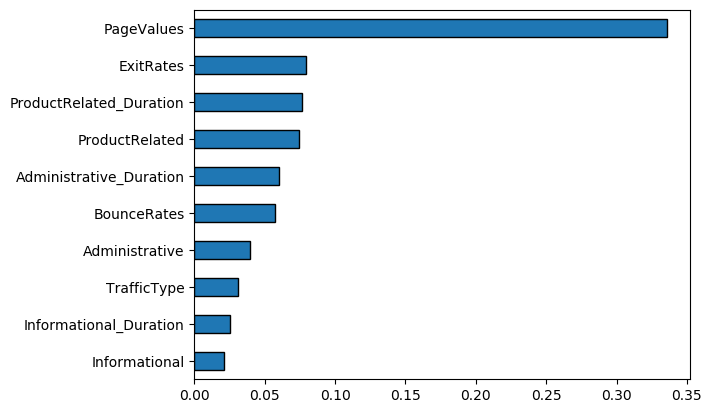
\includegraphics[width=8cm]{plots/feature_selection_random_forest_classifier.png}}

\capbtabbox{%
  \begin{tabular}{l|r}
Atribute                  & \multicolumn{1}{l}{Score} \\ \hline
ProductRelated\_Duration  & 877404.34                 \\
PageValues                & 175126.81                 \\
Administrative\_Duration  & 41754.84                  \\
Informational\_Duration   & 35059.78                  \\
ProductRelated            & 19317.29                  \\
Administrative            & 1133.97                   \\
Informational             & 357.98                    \\
Month\_Nov                & 223.55                    \\
VisitorType\_New\_Visitor & 115.34                    \\
Month\_May                & 55.00                     \\
SpecialDay                & 53.80                     \\
OperatingSystems\_3       & 48.55
\end{tabular}
}{%
  \caption{Top 10 features selected by SelectKBest}%
}
\end{floatrow}
\end{figure}

\newline
Looking at both models one can see that the two most important attributes are 'ProductRelated\_Duration' and 'PageValues.
Using the information from the two selections and through trial and error, by playing around with a few different attribute combinations, we have found the following top attributes:

\begin{itemize}
    \item Top 3: ['ProductRelated\_Duration', 'PageValues', 'Administrative\_Duration']
    \item Top 7: Top 3 + ['Informational\_Duration',  'ProductRelated', 'Administrative', 'Informational']
    \item Top 12: Top 7 +  ['BounceRates', 'ExitRates', 'PageValues', 'Month\_Nov', 'TrafficType' ]
\end{itemize}
Performance comparisons between the different Top attributes lists can be found in the following sections.



\subsection{K Nearest Neighbours Classifier}
Looking at \secref{fig:knn_wo_pre} one can see that using the most attributes leads to the best performance.  Interesting to note here, is that the best recall values were achieved when using k = 1 and thus only looking at the closest neighbour.

\begin{figure}
\begin{floatrow}
\ffigbox[\FBwidth][][]{\caption{Without Scaling (metric: Manhattan, weights: Uniform)}}
    {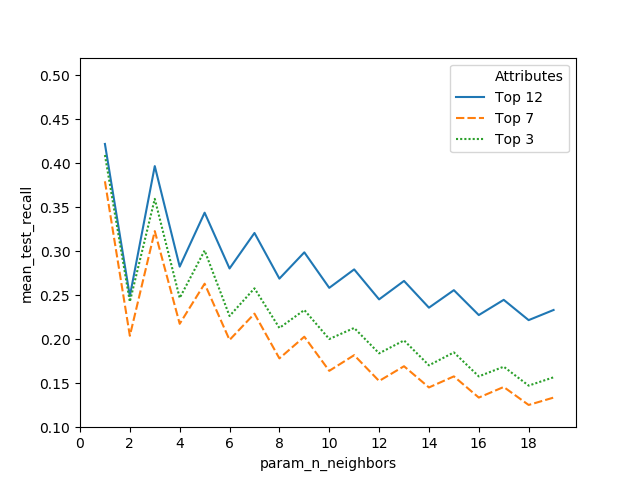
\includegraphics[width=6cm]{plots/knn_wo_preprocessing.png}\label{fig:knn_wo_pre}}
\ffigbox[\FBwidth][][]{\caption{With MinMax Scaling (metric: Uniform, Top 12 Attributes)}}
    {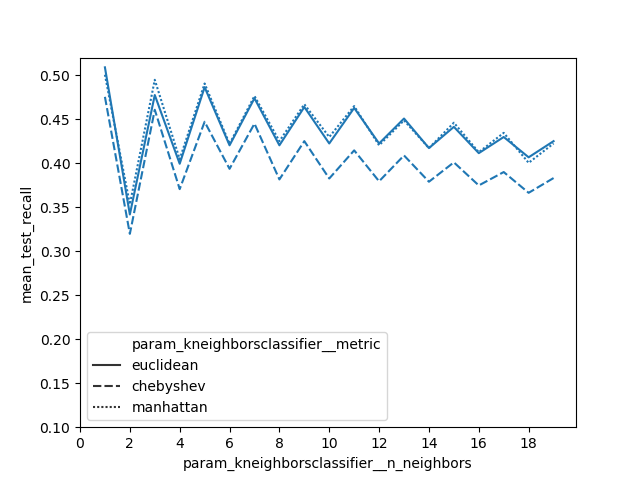
\includegraphics[width=6cm]{plots/knn_uniform_metric_comparison.png}\label{fig:knn_w_pre}}
\end{floatrow}
\end{figure}

As can be seen in \secref{fig:knn_w_pre} scaling the data leads to a best case improvement of around 0.07 compared to the unscaled data which only increases with increasing k. Another thing that scaling the data does, is reducing the overall decrease of the recall with changing k. This figure also shows that the euclidean and manhattan metric perform very similar for this dataset while the chebyshev performs slightly worse.


A general analysis beforehand showed that, while different weight parameters change how the recall values react to different k's, with \textit{uniform} being more sensitive compared to \texit{distance}, they do not change the best achievable values.

\subsection{Random Forest Classifier}
For Random Forest Classifier we have used GridSearchCV to try out a few different parameters like \texit{n\_estimators, max\_depth and the criterion}. \\
\newline
By doing a few pre tests and comparing how the criterion affects the recall value, we note that they lead to very similar results for this dataset. Since Gini is a tiny bit better than Entropy, it will be used for the other comparisons. \\
\newline

\begin{figure}
\begin{floatrow}
\ffigbox[\FBwidth][][]{\caption{Comparison of \textit{n\_estimators} for different \textit{max\_depth} values}}
    {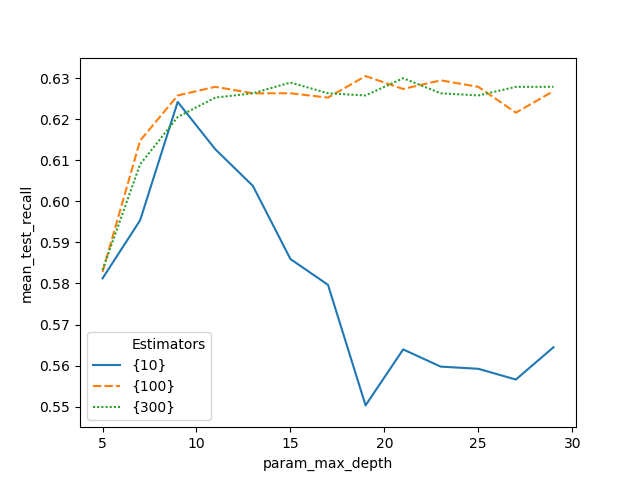
\includegraphics[width=6cm]{plots/rfc_n_estimators_comparison.png}\label{fig:rf_n_estim}}
\ffigbox[\FBwidth][][]{\caption{Scaling vs No Scaling comparison (100 Trees)}}
    {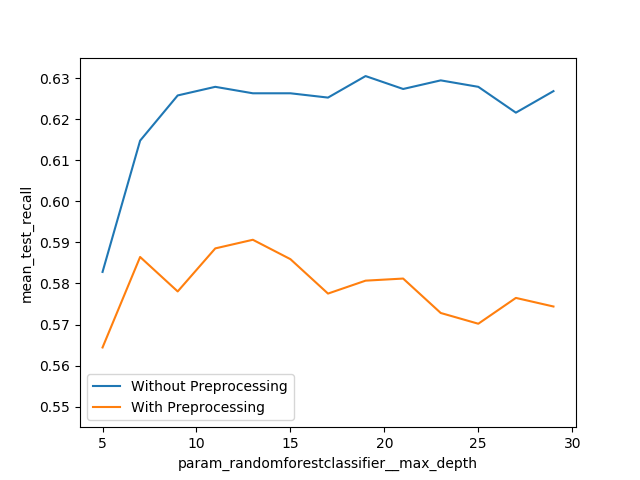
\includegraphics[width=6cm]{plots/rfc_preprocessing_comparison.png}\label{fig:rfc_pre}}
\end{floatrow}
\end{figure}

Looking at the different n\_estimators in \secref{fig:rf_n_estim} we can see that a higher n\_estimators makes up for the overfitting which will be achieved by having a too high max\_depth value. This makes sense as the amount of trees within a forest is a good way to control overfitting. On the other hand after a certain point it makes no difference if there are 100 or 300 trees.

As trees are very robust and thus do not need Preprocessing most of the time, applying a MinMaxScaler to our data actually led to worse values which is visualized in \secref{fig:rfc_pre}.

\subsection{Multi-Layer Perceptron Classifier}
\image{plots/mlp_np_comparision.png}{Comparison of different models and activation functions}{\label{mlp}}

\subsection{Conclusion}

\subsubsection{Preprocessing vs No-Preprocessing}
To be able to look at more than just the numerical values, \texit{No-Preprocessing} in this case stands for the data after the general Preprocessing (One Hot Encoding, remove Missing values, ...) mentioned in \secref{GenPrepro} has been done. We compare the unpreprocessed data with the data after MinMax scaling and after introducing a new feature by weighting the outliers.

% TODO

\begin{table}[h]
\begin{center}
\begin{tabular}{|l|l|l|}
\hline
                       & Preprocessing & No-Preprocessing \\ \hline
KNeighborsClassifier   & x        & x           \\ \hline
RandomForestClassifier & x        & x           \\ \hline
MLPClassifier          & x        & x           \\ \hline
\end{tabular}
\caption{Comparision of accuracy of different techniques with- and without preprocessing}
\end{center}
\end{table}

\subsubsection{Holdout vs Cross Validation}
By comparing the achieved holdout and cross validation values we can see that the holdout method leads to better results. This is a possibility since the training split is randomly chosen, which plays a big part.

\begin{table}[h]
\begin{center}
\begin{tabular}{|l|l|l|}
\hline
                       & Holdout & Cross Validation \\ \hline
KNeighborsClassifier   & 0.5236  & 0.5089           \\ \hline
RandomForestClassifier & 0.5863  & 0.5817           \\ \hline
MLPClassifier          & x  & x           \\ \hline
\end{tabular}
\caption{Comparision of accuracy of holdout versus cross-validation}
\end{center}
\end{table}

\begin{table}[h]
\begin{center}
\begin{tabular}{|l|l|l|l|l|l|}
\hline
                       & Accuracy & Precision & Recall & F1     & Runtime (sec) \\ \hline
KNeighborsClassifier   & 0.8525   & 0.5483  & 0.5089 & 0.5213 & 0.043416        \\ \hline
RandomForestClassifier & 0.8982   & 0.7187    & 0.5817   & 0.6408   & 1.0573        \\ \hline
MLPClassifier          & x   & x    & x   & x   & x        \\ \hline
\end{tabular}
\caption{Comparison of different performance metrics and runtimes}
\end{center}
\end{table}

\end{document}